\section{User interface design}
In this section are presented some mockups of the main features and related user interfaces the system is supposed to offer to the user and to the customer care through the proper web-based application.
\subsection{User app}
The user app must have a charming and intuitive user interface in order to provide a easy-to-use experience to the user. The interface must be optimized for mobile devices even if the application is accessible and must be usable from every web browser on different size devices.

\subsubsection{Login page}
Simple initial page for the application to allow the user to authenticate to the system through username and password. A new user can access the registration process through the \emph{New User} button. \\
As specified in the requirements document, thist page also allows a guest user or a \emph{banned} registered user to access to customer care contact information through the \emph{Contact us} button. \\
If a user is not recognized or is banned an error alert is shown when credential are submitted.

	\begin{figure}[h]
			\centering
			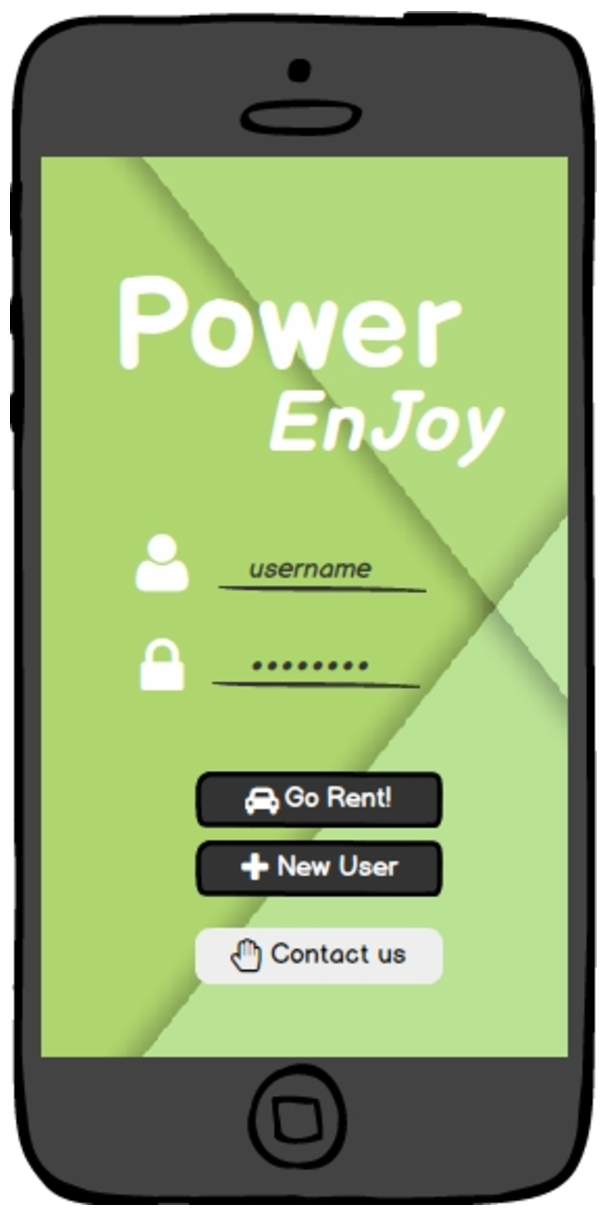
\includegraphics[width=0.4\linewidth]{mockups/loginPage}
			\caption{
				\label{fig:loginPage} 
				\emph{Login page} mockup
			}
		\end{figure}
		

\subsubsection{Home page}
The home page shows to a logged user all the possible functionalities provided from the app:
\begin{itemize}
	\item See available cars and reserve one of them (eventually with the \emph{money saving option})
	\item Unlock a car (disabled button in the mockups, it would be active only if there is an active reservation for the registered user logged in)
	\item See user's information and edit them
	\item See user's rent history
	\item See user's payment history
	\item Show customer care contact information
\end{itemize}

This page shows also the user's name to ensure to the user he has been correctly recognized by the system and to make the interface more customized. \\

The icon in the right corner, from this page, brings the user to the functionality of see available cars; on all other pages (without the orange position icon) it brings the user to this page: the home page.

	\begin{figure}[h]
			\centering
			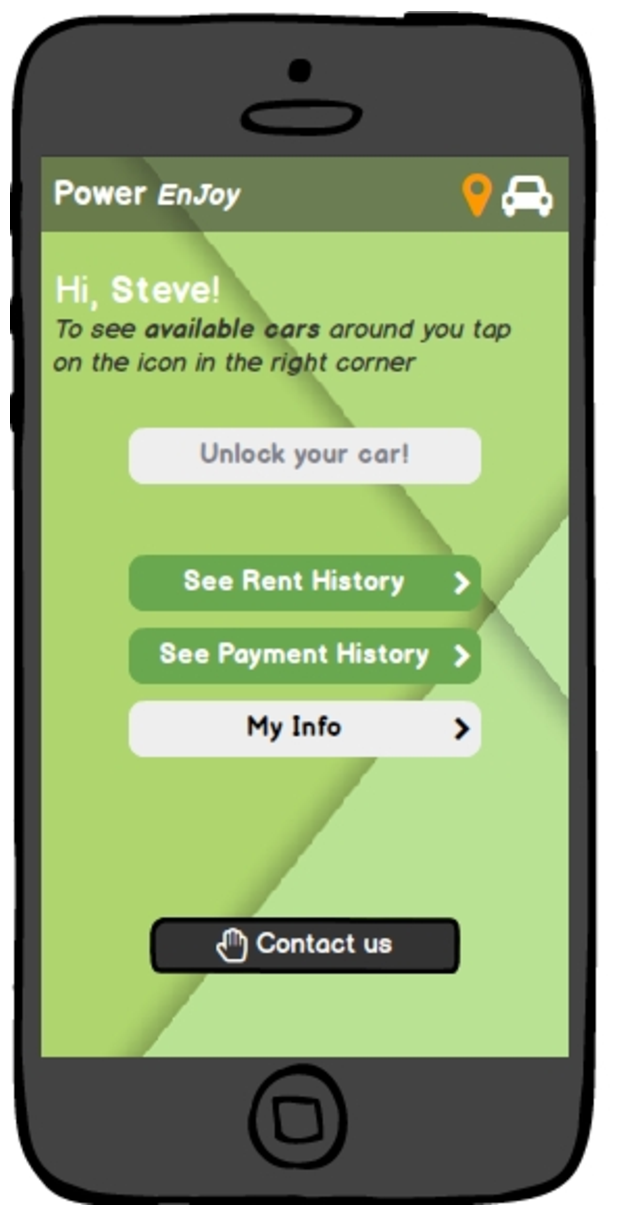
\includegraphics[width=0.4\linewidth]{mockups/homePage}
			\caption{
				\label{fig:homePage} 
				\emph{Home page} mockup 
			}
		\end{figure}
		
\subsubsection{See available cars}
Accessing to the see available cars functionality, as described in the requirements document, the system asks to the user if he wants to search car nearby his actual position (using GPS position of user's device) or he wants to insert a different position from which starting the research. \\

The \emph{Use GPS} allows the user to choose the first option skipping other interactions on this page. \\

If the user chooses the second option, he is supposed to insert an address location (e.g. 34 Maria Victoria Lane, London) before pushing the \emph{Search} button; the system will resolve that address as a GPS location displaying an error message if it could not done it. \\

The \emph{Cancel} button allows the user to return to the home page. \\

The system searches for available cars (nearby the position given by the user or retrieved by the GPS) and displays a map with available cars on their actual position. Blue circled cars are actually plugged on a charging station, all others car are green circled.\\

The map is interactive and the user can move around the actual position. \\

	\begin{figure}[h]
			\centering
			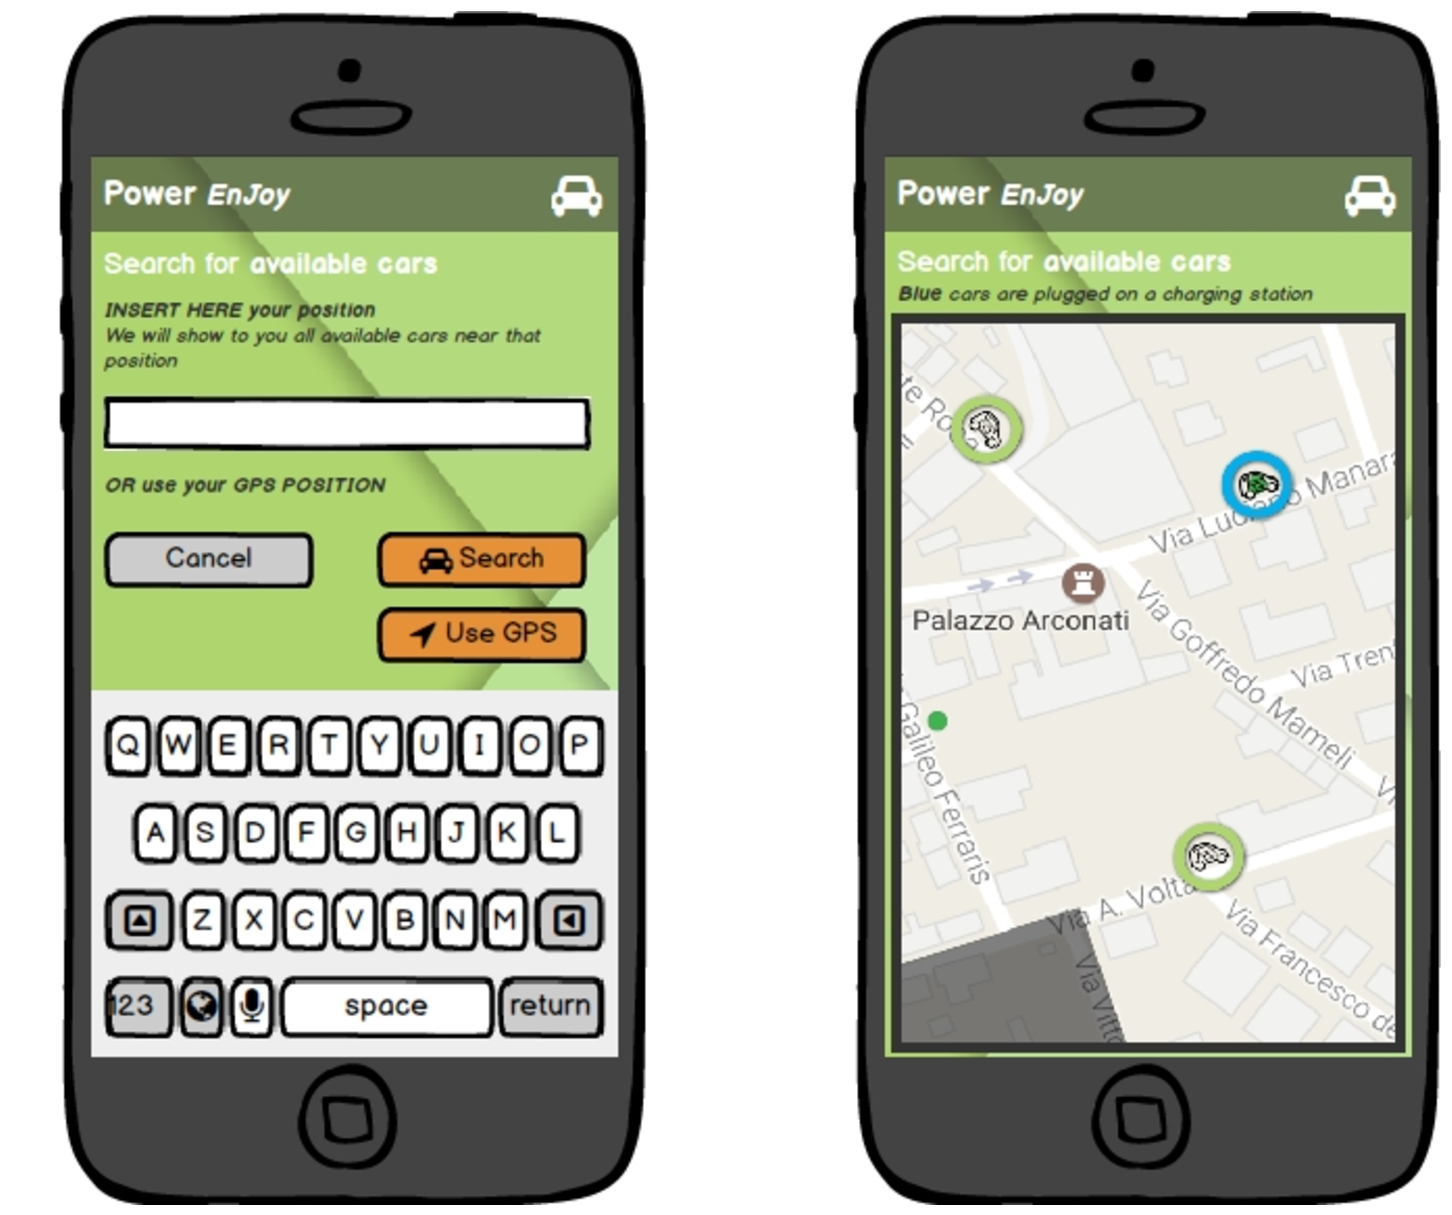
\includegraphics[width=0.9\linewidth]{mockups/findCar}
			\caption{
				\label{fig:searchCar} 
				\emph{See available cars} mockup
			}
		\end{figure}

\subsubsection{Reserve a car}

From the page showing available cars on the map, a user tapping on a car could access information about it, in particular:
\begin{itemize}
	\item Model of the car
	\item License number of the car
	\item The battery percentage level of the car
\end{itemize}

When the user taps on a car the circle around it becomes orange, to give a feedback on the tap to the user, and a box appears on the screen. Through it the user can access the aforementioned info about the car and reserve the selected car. \\

Before clicking the \emph{Reserve it!} button the user has the possibility to choice if he wants or not to enable the \emph{money saving option} through an on/off toggle.\\

If a user has already an active reservation or the selected car has been reserved while the user navigates on the map an error message is displayed.\\

\begin{figure}[h]
			\centering
			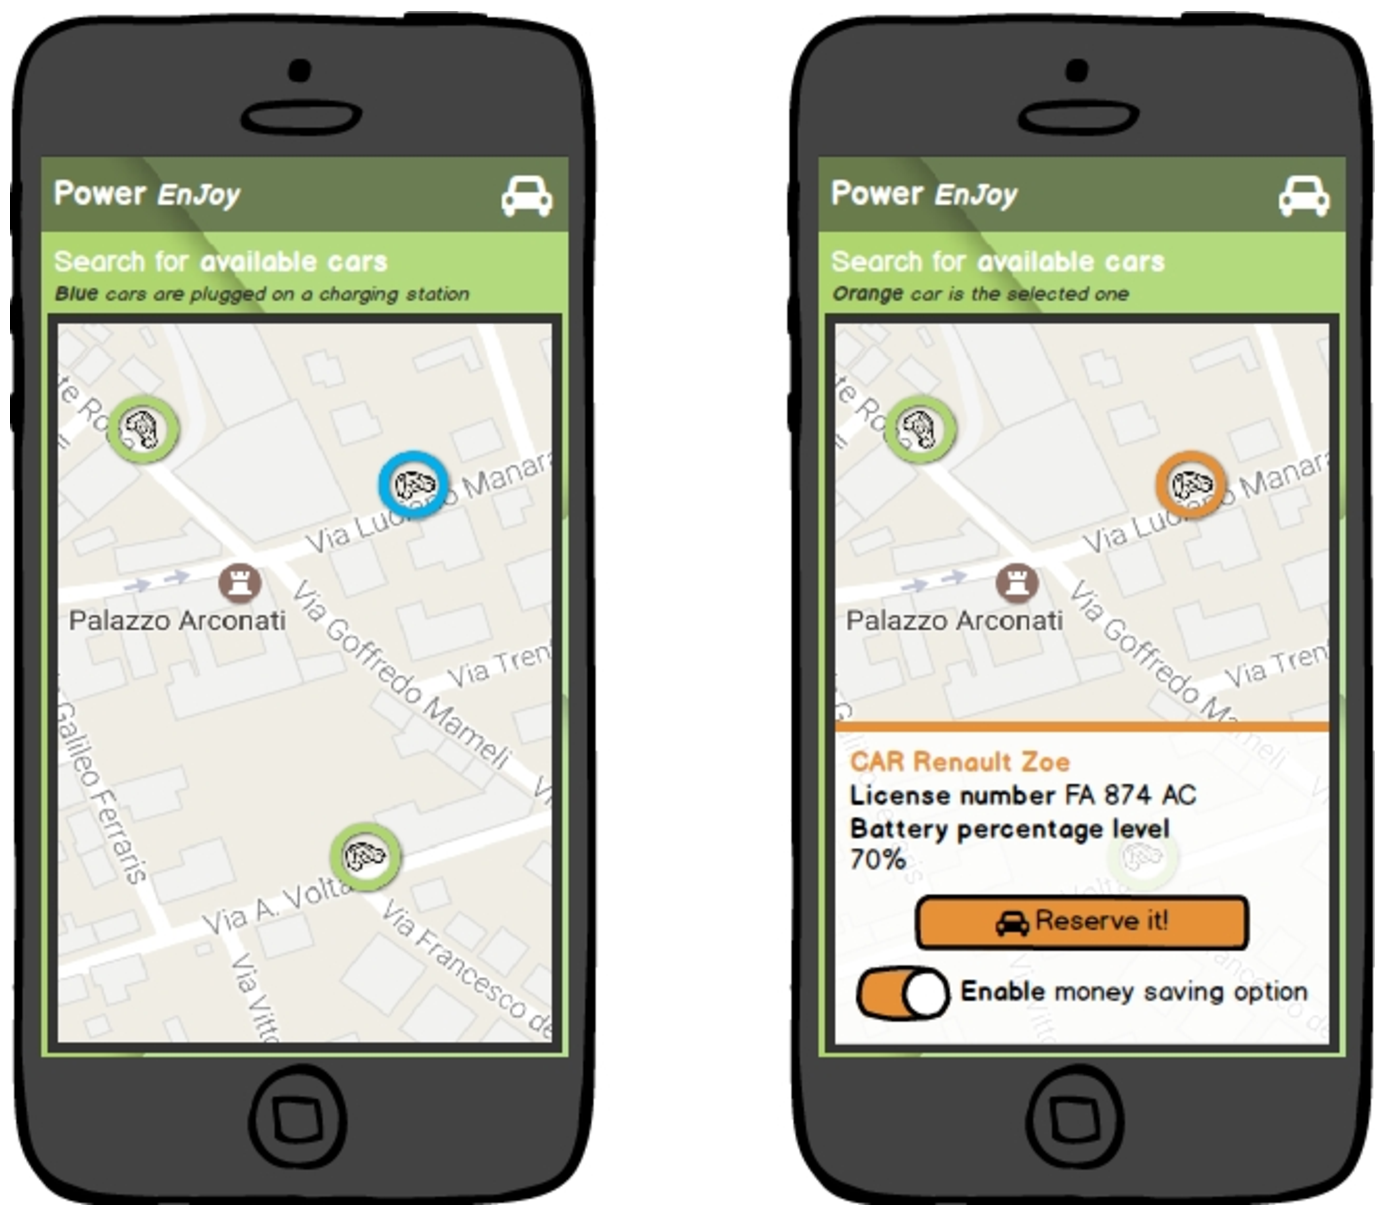
\includegraphics[width=0.9\linewidth]{mockups/reserveCar}
			\caption{
				\label{fig:reserveCar} 
				\emph{Reserve a car} mockup
			}
		\end{figure}
		
\subsubsection{Money saving option}

If an user enables the \emph{money saving option} while reserving a car, the system shows him a dedicated page to accomplish the reservation with the option. On this page the user must insert the planned destination of his rent in order to give to the system the possibility to calculate the charging station the user must leave the car plugged in to get the discount.\\

A brief description of the \emph{money saving option} is offered to the user to clarify why the system is asking him his planned destination. \\

The user is supposed to insert an address location (e.g. 34 Maria Victoria Lane, London) before pushing the \emph{Confirm} button; the system will resolve that address as a GPS location displaying an error message if it could not done it. \\

If the address inserted by the user is correctly processed the system notifies the user with the charging station (number and address) 
the user must leave the car plugged in to get the discount. \\

The \emph{Cancel} button allows the user to go back on the map, for example to make the reservation without enabling the \emph{money saving option}.\\

\begin{figure}[h]
			\centering
			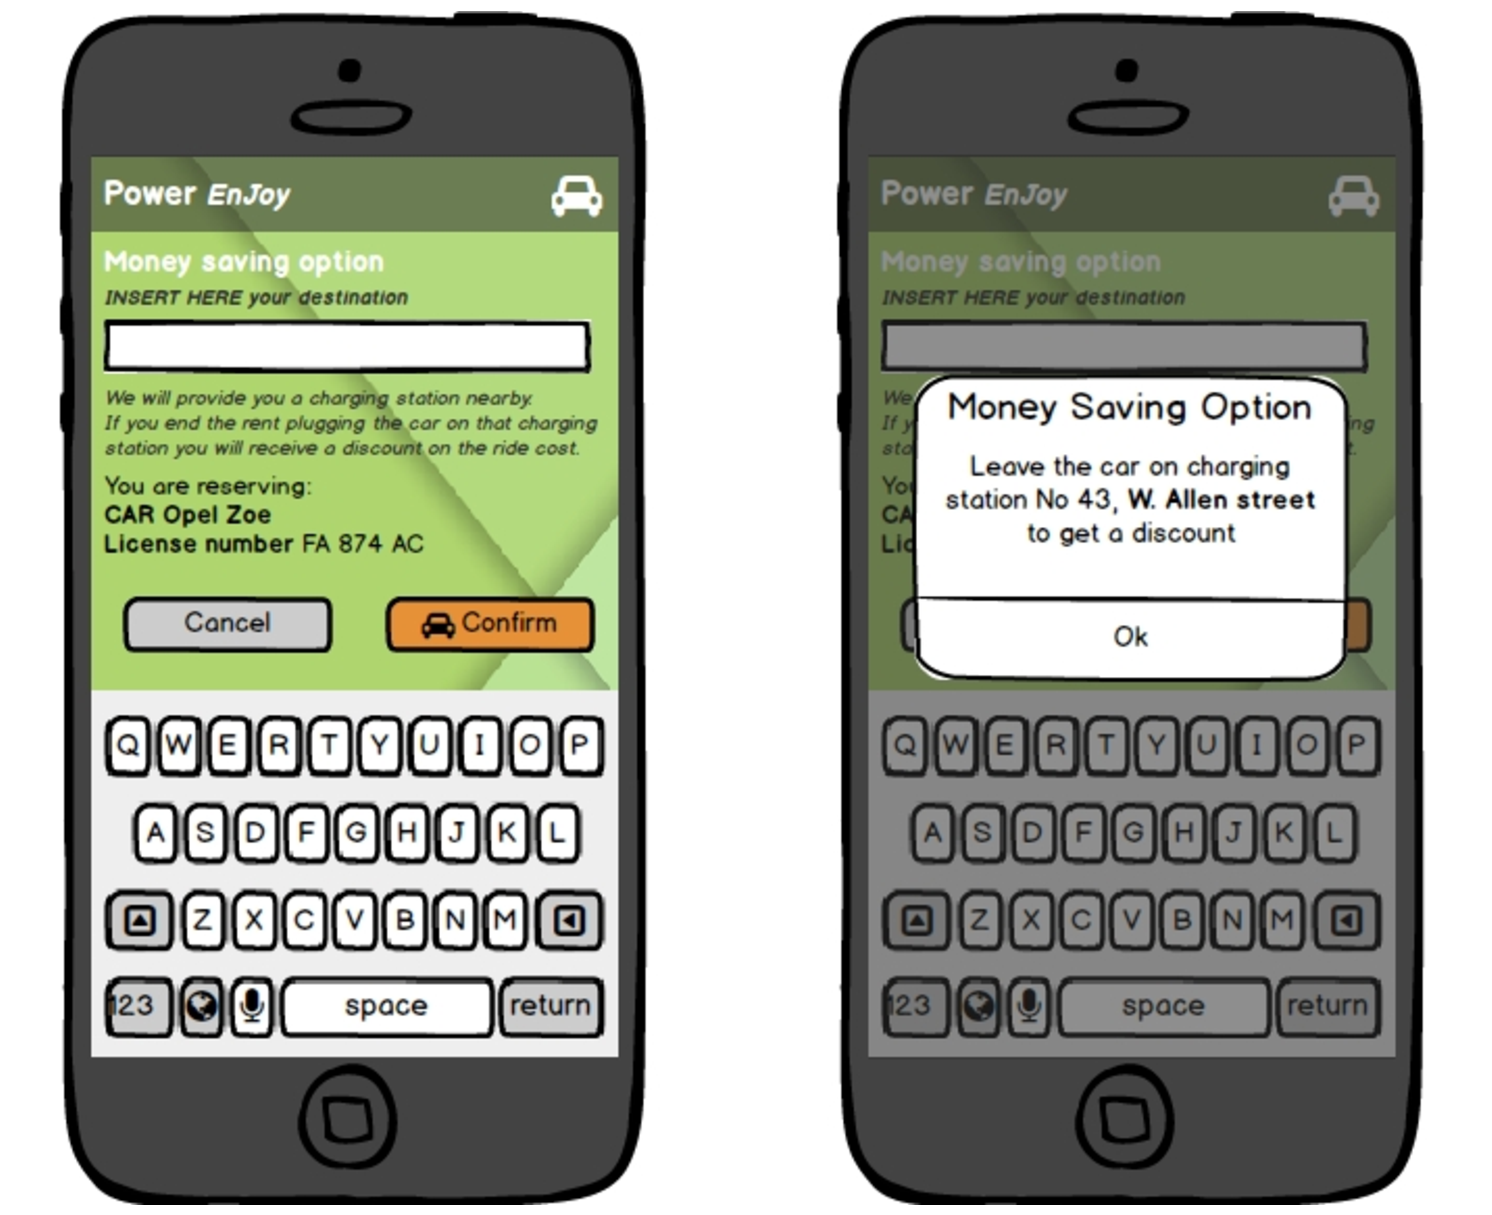
\includegraphics[width=0.9\linewidth]{mockups/moneySavingOption}
			\caption{
				\label{fig:msOption} 
				\emph{Money saving option} mockup
			}
		\end{figure}

\subsubsection{Unlock a car}

\begin{figure}[h]
			\centering
			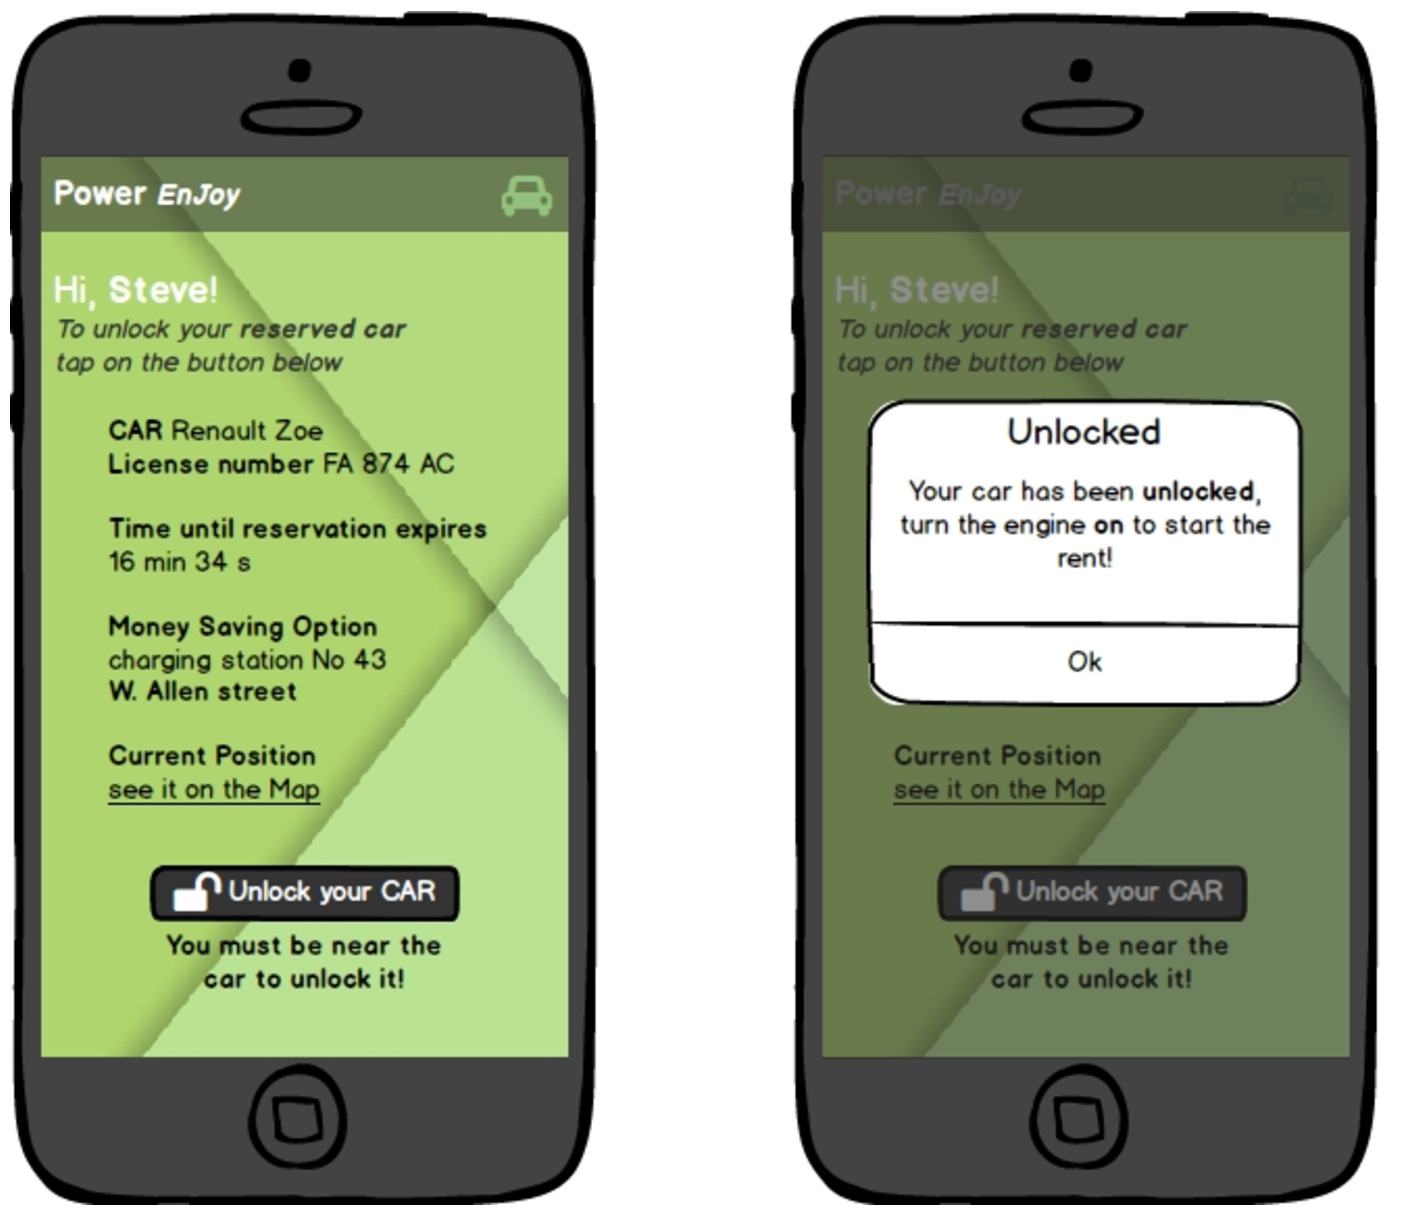
\includegraphics[width=0.9\linewidth]{mockups/unlockCar}
			\caption{
				\label{fig:unlockCar} 
				\emph{Unlock a car} mockup
			}
		\end{figure}
		
\subsection{Customer care app}